\chapter{Saber: delegating transport layer security to browsers}
\label{ch:saber}

\section{Introduction}
\label{sec:intro-saber}

Transport Layer Security (TLS) is a cryptographic protocol designed to provide
end-to-end communication security between two parties, even in the presence of
active man-in-the-middle adversaries~\cite{RFC5246}. It has since become the
standard for providing secure communication on the Internet and is used for
most sensitive applications, including online banking, email, instant
messaging, shopping, etc. Usage of TLS is most commonly seen in securing web
traffic in the form of HTTPS~\cite{RFC2818}. When implemented correctly, HTTPS
guarantees confidentiality, integrity, and authenticity of all web
communication between two parties. On the web, there are additional mechanisms
such as \emph{strict transport security} (HSTS)~\cite{RFC6797}, \emph{public
key pinning} (HPKP)~\cite{RFC7469}, \emph{online certificate status protocol}
(OCSP) stapling, and \emph{certificate transparency} (CT)~\cite{RFC6962}, that
improve the security of HTTPS. However implementing HTTPS and all these
supporting security mechanisms correctly has proven to be a challenge for many
applications.

While browsers are not free from TLS bugs, theier implementations of network
security protocols are regarded as the state of the art. Browser vendors have
further been the pioneers of modern HTTPS standards and are the first to
implement them into practice. Previous work has found that non-browser
applications have struggled with validating TLS certificates~\cite{dangerous}.
As this thesis shows, many of the applications lag behind in other web security
practices such as HSTS, HPKP, and certificate revocation checking. Despite
this, usage of non-browser software such as package managers, command-line HTTP
clients, and language specific request libraries, is prominent. These
applications and libraries support communication atop TLS and hence provide the
impression of giving security to the user, but they fail to live up to that
promise. In contrast, we find that browsers such as Chrome and Firefox
implement not only secure validation of TLS certificates in general, but also
implement mechanisms such as HSTS, HPKP, verification of revoked
certificates, and have dynamic protection against identified malware and
dangerous binaries~\cite{safe-browsing}. They are also better at communicating
security warnings to the user in a transparent manner~\cite{improve-warnings}.

The issues with improper implementation of TLS for non-browser applications are
due to both the complexity of the protocol, lack of general understanding of
TLS, and not having the same security expertise and engineering resources for
development as browsers do. Solving these issues would be a monumental task and
would require widespread education of the importance of properly implementing
communication security. along with the expense of recruiting security experts
for every application that supports HTTPS. This may not be feasible for several
applications that are maintained by individual developers but are nonetheless
popular.

We propose a new way to build command-line HTTP clients that allows developers
to use the TLS protocol for web security but does not require the expertise
needed to implement TLS and HTTPS security practices correctly. Our method
involves delegating the handling of connection security to browsers, so the
non-browser application deals only with application layer logic. This allows
non-browser applications to get connection security ``for free'' from browsers.
This also lets them take advantage of any mechanisms that browsers implement to
harden TLS security (such as HSTS, HPKP, etc.). We have built a prototype
version of wget in this fashion. Our secure wget (\emph{swget}) application is
able to validate proper TLS connections without writing any code that requires
a deep knowledge of the TLS protocol, and further provide modern HTTPS security
guarantees that only browsers typically provide.

This chapter is organized as follows: In \Cref{sec:background-saber}, we
discuss the background material related to TLS and HTTPS, the various existing
problems with the ecosystem and how browsers have taken steps to solve them. In
\Cref{sec:problems-saber} we look at some non-browser applications, in
particular \emph{wget} to see how they compare to modern browsers in terms of
connection security. In \Cref{sec:solution-saber}, we present the design of a
library that delegates connection security to the browser. In
\Cref{sec:swget-saber}, we present \emph{swget} as a prototype implementation
of wget that provides better connection security by delegating TLS to browsers.
In \Cref{sec:conclusion-saber}, we conclude and discuss related work.


\section{Background}
\label{sec:background-saber}

In this section, we present a brief description TLS, HTTPS, and additional security
mechanisms that harden the HTTPS ecosystem.

\subsection{TLS}
Transport Layer Security (TLS) is a cryptographic protocol that has been
established as the standard method of secure, encrypted communication over the
Internet~\cite{RFC5246}. TLS aims to provide \emph{Authenticated Encryption} which requires the
following key properties-
\begin{itemize}
  \item \textbf{Confidentiality:} All communication between two parties is
    encrypted such that no information about the contents of the communication
    is leaked to an adversary.

  \item \textbf{Integrity:} An adversary must not be able to change the
    contents of the communication between the two parties in any way.

  \item \textbf{Authenticity:} The two communicating parties can verify the
    identity of each other (typically only the client verifies the server
    identity) through a certificate signed by a \emph{trusted third-party}, and
    ensure that the messages exchanged are from each other. As such, an
    adversary cannot pretend to be one of the comunicating parties.
\end{itemize}

TLS provides these security guaranties underneath the application layer.
Several application layer protocols such as HTTPS, IMAPS, XMPP, and SMTP use
TLS to provide end-to-end security.

\subsection{HTTPS}
HTTPS (or ``HTTP over TLS'') is a protocol which secures HTTP traffic within a
connection encrypted by the TLS protocol~\cite{RFC2818}. It is mainly used for
authenticating a website and securing communication between the website and its
users. This is done with the use of server certificates~\cite{RFC5280}.
In a normal HTTPS connection, when a client makes a request over HTTPS to some
website, the server presents the client with a certificate signed by some
certificate authority. This certificate authority may not directly be trusted
by the client but may instead be trusted by another entity that the client may
trust. The server also responds with a chain of trust listing all the CAs that
are part of the chain connecting to a root CA that the client trusts.

A client needs to validate the certificate's credentials and determine the
validity of the certificate. A client may find the certificate to be invalid in
cases when it's expired, has a mismatching common name field, is revoked, uses a
weak signature algorithm, etc. We list several different types of client
behavior for certificates in \Cref{tab:results-table-saber}.

\subsection{Strict Transport Security}
While HTTPS protects users from active man-in-the-middle attackers, the
protection only applies if the client actually makes an HTTPS web request.
Browser extensions such as \emph{HTTPS Everywhere} force every request to be
HTTPS, but with a large portion of the web only accessible over
HTTP~\cite{https-ecosystem}, such an extension is infeasible for an average
user and would block access to a significant portion of the Internet for users.

Secure connection to a domain that does serve over HTTPS can only be guaranteed
if the initial web request made by the client was over HTTPS. Unencrypted HTTP
requests and responses can be modified freely by an active man-in-the-middle
attacker. Even if a web server redirects from HTTP to HTTPS for partial or all
of the web requests that it serves, an active man-in-the-middle attacker could
intercept that unecnrypted redirect response and replace it with a forged
accept-response pretending to be the server. As a result, the attacker could
make it so that the client never actually switches to an HTTPS connection and
remains vulnerable. This class of attacks is commonly known as \emph{SSL
Stripping}~\cite{sslstrip}.

To combat this problem, servers should also serve a
\emph{Strict-Transport-Security} (HSTS) header as part of the response that
instructs the client to only visit the website over HTTPS
connection~\cite{RFC6797}. A client that respects this HSTS policy would
automatically upgrade all HTTP requests made by the user to HTTPS before
sending the request over the network. As long as the client can guarantee a
secure connection with a domain once and receive an HSTS header, all future
communication within a designated timeframe to that domain is protected. HSTS
headers also need to provide a \emph{max-age} policy that determines how long a
client enforces the HSTS policy. This policy is continuously updated every time
an HSTS header is received, so if a client visits the same website again within
the expiry period, the client stays protected. Otherwise, the client loses
protection when the max-age policy expires and protection is resumed once the
client receives a fresh HSTS header from securely connecting to the domain
again. The \emph{max-age} policy allows websites to switch back to HTTP
connections should they choose to do so in the future. Without a max-age
policy, a client wouldn't be able to communicate over HTTP with the server
again once it has received an HSTS header.

HSTS relies on the \emph{Trust On First Use} (TOFU) principle to harden
protection. Today, browsers actually ship with preloaded list of domains that
have HSTS protection turned on by default so that users gain HSTS protection
even before they establish a single secure connection. Any domain owner can
apply to be a part of this list and the process has seen significant adoption
since it was automated by Chrome~\cite{hstspreload}.


\subsection{Public Key Pinning}
The current HTTPS Public Key Infrastructure relies on trusting all the root CAs
and by extension, all intermediate CAs trusted by root CAs. This raises the
concern that if one of the CAs was coerced or compromised by some adversary,
then that CA could issue a valid rogue certificate for some website without the
permission of the owner of the website. This rogue certificate would be trusted
by any user that trusts the CA that generated it. Previous work has shown that
certificate authorities can be falsely tricked into issuing rogue certificates
and in 2010, a commercial software was available for sale to government
agencies to use rogue certificates for intercepting
traffic~\cite{commercial-government}. HTTPS and HSTS alone do not protect from
this kind of interception.

Instead, \emph{HTTP Public Key Pinning} (HPKP) solves this problem by allowing web
servers to serve an HTTP header over HTTPS that lists the hashes of the
complete \emph{Subject Public Key Info} field of a certificate for each public key
that the domain owner wishes to use to establish a TLS connection. A client
that respects the HPKP policy must ensure that while establishing a TLS
connection with a website for which there is a cached HPKP entry, at least one
key in the certificate chain matches a key stored in the pin set~\cite{RFC7469}.

This allows a domain owner to pin only their own keys. In the case that the
owner chooses to only pin leaf-level keys generated by the owner themselves, no
CA would be able to generate a rogue certificate for the domain that a client
that has already had the keys pinned. The owner can also choose to pin the
public keys for specific CAs that they trust (over all CAs), still reducing the
surface area for attackers that compromise CAs.

Similar to HSTS, HPKP headers also specify a \emph{max-age} policy which
determines how long a client should remember the pinned key. This value also
keeps getting continuously updated if the client receives the header again
before the policy expires. HPKP headers are not very commonly seen from
websites but both Firefox and Chrome provide support for it. Browsers also
ship preloaded HPKP lists similar to HSTS that provide this protection
by default.

\subsection{Certificate Revocations}
In the case that a domain's private key gets leaked (due to server compromise,
phishing, etc.) any certificates that were issued for the corresponding public
key need to be revoked. Both registering a certificate as revoked and checking
the revocation status of a certificate have been tricky challenges for the
server and client respectively~\cite{revocation-measurement}.

One way for checking revoked certificates is to maintain a Certificate
Revocation List (CRL) for all revoked certificates which the clients could use
to validate the certificate~\cite{RFC5280}. This list needs to be continuously
updated with the latest revocations and clients need to be able to check the
revocation status of a certificate dynamically. In a situation where a client
is unable to access the revocation list (for example if an adversary runs a
denial of service attack that prevents the client from contacting the server),
then no further operations that depend upon the validation of the certificate
can take place.

Online Certificate Status Protocol (OCSP) is an Internet protocol used to
communicate the revocation status of x509 certificates~\cite{RFC2560}. The
protocol works similarly to CRLs but require less bandwidth on the client. A
client requests the status of a certificate from an OCSP server, which responds
whether the certificate is revoked or not. OCSP still has the same denial of
service issues as CRLs and many clients tend to accept a certificate if they
cannot successfully get an OCSP response. To address this issue, the original
server that presents the certificate can make a request to the OCSP server and
staple the OCSP response along with the original certificate, which the client
can verify offline. This is known as OCSP stapling and many web servers support
it today (although only about 9\% of TLS connections use it as of
2015)~\cite{onecrl}.

Despite OCSP stapling, an attacker that can compromise a server can simply
serve the certificate without a stapled OCSP response which the client may
accept. Website owners therefore have an option to issue a certificate with a
``Must-Staple'' flag~\cite{must-staple}. If a client sees this flag in the
certificate, the client must not accept the certificate without a stapled
response. This is respected by Chrome and Firefox.

Chrome and Firefox have also introduced offline CRLs that they push to user's
browsers during updates~\cite{onecrl, crlsets}. This is primarily used for
serious incidents (say if an intermediate CA gets compromised) to push
emergency updates to the CRLs maintained by the client.


\section{Issues with non-browsers}
\label{sec:problems-saber}

TLS is a complicated protocol to implement correctly and the configuration
options in TLS libraries are difficult to understand. Several non-browser
softwares have been shown to be insecure against a network attacker not due to
using an incorrect protocol, or a broken library, but rather due to incorrect
certificate validation arising out of mistakes when configuring TLS options for
their application~\cite{dangerous}.

Further, even a correct implementation of TLS does not protect these
applications from SSL stripping, rogue certificates, and revocations, unless
all the additional mechanisms such as HSTS, HPKP, and OCSP stapling are also
implemented by the application. In our experiments with wget, curl, and the
standard request libraries for Python and Node.js, we found that only wget
supports HSTS and has very limited and manual support for public key-pinning.
None of the four HTTP clients threw any form of error or warning for a revoked
certificate and the request libraries for Python and Node.js, and curl do not
have any support for HSTS and HPKP.

Wget provides support for HSTS, but upon investigation, we found that wget was
not updating the expiration time for HSTS entries every time it received a
valid HSTS header with a valid max-age policy. This breaks the continuity
policy of HSTS which is supposed to maintain a secure HSTS entry as long as
user visits the domain frequently (i.e. within the specified max-age period).
If a domain provides an HSTS max-age policy of 1 day, then the wget client
would be vulnerable to interception at least once a day even if the developer
visits the domain multiple times within that period. We reported this issue to
wget which was then promptly fixed~\cite{wgetbug}.

\subsection{Certificate validation results}
We tested the behavior of 6 different HTTP clients (2 command-line tools, 2
language request libraries, 2 browsers) when presented with 27 different types
of certificates. The complete results are presented in \Cref{tab:results-table-saber}.
Explanation of different types of certificates we tested-
\begin{enumerate}
  \item \textbf{Expired.} The certificate has an expiration date in the past.
  \item \textbf{Wrong Host.} The certificate is not valid for the website that
    presented it and should be rejected.
  \item \textbf{Self Signed.} The certificate is signed by the identity it
    certifies and should be rejected.
  \item \textbf{Untrusted Root.} The root authority is not trusted by the
    client and should be rejected.
  \item \textbf{Revoked.} The certificate used to be valid but was revoked by
    the owner and should be rejected.
  \item \textbf{Pinning Test.} A different certificate has been pinned (via an
    HPKP header) and so this certificate should be rejected.
  \item \textbf{Incomplete Chain.} The certificate chain presented is
    incomplete. Browsers accept this certificate since the incomplete chain was
    sufficient to establish trust.
  \item \textbf{SHA1 Intermediate.} One of the certificates in the chain was
    signed using a SHA1 signing algorithm and should be rejected.
  \item \textbf{1000/10000 Subject Alt Names.} The certificate provides 1000 or
    10000 alternate subject names. This behavior is acceptable.
  \item \textbf{RC4-MD5, RC4, 3DES, Null.} These are different types of weak
    cipher suites used by the respective certificates (and no cipher suite in
    the Null case). All of these should be rejected.
  \item \textbf{DH480, DH512, DH1024, DH2048.} These are the different types of
    Diffie-Hellman key exchange algorithms used by the connection. Only DH2048
    is currently considered completely secure.
  \item \textbf{DH Small Subgroup, DH Composite.} If the key exchange was
    performed with a small or non-prime subgroup, then security cannot be
    guaranteed and these connections should be rejected.
  \item \textbf{Invalid Expected SCT.} The certificate for this site uses a CA
    that Chrome requires valid Signed Certificate Timestamps (SCTs) for, but
    contains an invalid SCT. Only Chrome enforces this check.
  \item \textbf{Superfish, eDellRoot, DSD Test Provider.} These are certificates
    issued known bad certificate authorities and should be rejected.
\end{enumerate}

\begin{footnotesize}
\begin{longtabu} to \textwidth {||c | c c c c c c ||}
  \caption[Certificate error testing]{Behavior of different clients when
  presented with different certificates. A green entry indicates that behavior
  is safe. A red entry indicates that the behavior is not ideal.}
  \label{tab:results-table-saber} \\
  \hline \multicolumn{1}{||c|}{\textbf{Certificate}} &
         \multicolumn{1}{c}{\textbf{wget}} &
         \multicolumn{1}{c}{\textbf{curl}} &
         \multicolumn{1}{c}{\textbf{python}} &
         \multicolumn{1}{c}{\textbf{node}} &
         \multicolumn{1}{c}{\textbf{firefox}} &
         \multicolumn{1}{c||}{\textbf{chrome}} \\ \hline 
  \endfirsthead

  \multicolumn{7}{c}%
  {{\bfseries \tablename\ \thetable{} -- continued from previous page}} \\
  \hline \multicolumn{1}{||c|}{\textbf{Certificate}} &
         \multicolumn{1}{c}{\textbf{wget}} &
         \multicolumn{1}{c}{\textbf{curl}} &
         \multicolumn{1}{c}{\textbf{python}} &
         \multicolumn{1}{c}{\textbf{node}} &
         \multicolumn{1}{c}{\textbf{firefox}} &
         \multicolumn{1}{c||}{\textbf{chrome}} \\ \hline 
  \endhead

  \hline \multicolumn{7}{|r|}{{Continued on next page}} \\ \hline
  \endfoot

  \hline \hline
  \endlastfoot
    Expired & \RejectedG & \RejectedG & \RejectedG & \RejectedG & \RejectedG & \RejectedG\\
    Wrong Host & \RejectedG & \RejectedG & \RejectedG & \RejectedG & \RejectedG & \RejectedG\\
    Self Signed & \RejectedG & \RejectedG & \RejectedG & \RejectedG & \RejectedG & \RejectedG\\
    Untrusted Root & \RejectedG & \RejectedG & \RejectedG & \RejectedG & \RejectedG & \RejectedG\\
    Revoked & \AcceptedR & \AcceptedR & \AcceptedR & \AcceptedR & \RejectedG & \RejectedG\\
    Pinning Test & \AcceptedR & \AcceptedR & \AcceptedR & \AcceptedR & \RejectedG & \RejectedG\\
    Incomplete Chain & \RejectedG & \AcceptedR & \RejectedG & \RejectedG & \AcceptedR & \AcceptedR\\
    SHA1 Intermediate & \AcceptedR & \AcceptedR & \AcceptedR & \AcceptedR & \RejectedG & \RejectedG\\
    1000 Subject Alt Names & \AcceptedG & \AcceptedG & \AcceptedG & \AcceptedG & \AcceptedG & \AcceptedG\\
    10000 Subject Alt Names & \RejectedR & \AcceptedG & \RejectedR & \RejectedR & \RejectedR & \RejectedR\\
    RC4-MD5 & \AcceptedR & \RejectedG & \RejectedG & \RejectedG & \RejectedG & \RejectedG\\
    RC4 & \AcceptedR & \RejectedG & \RejectedG & \RejectedG & \RejectedG & \RejectedG\\
    3DES & \AcceptedR & \AcceptedR & \RejectedG & \RejectedG & \AcceptedR & \AcceptedR\\
    Null & \RejectedG & \RejectedG & \RejectedG & \RejectedG & \RejectedG & \RejectedG\\
    DH480 & \RejectedG & \RejectedG & \RejectedG & \RejectedG & \RejectedG & \RejectedG\\
    DH512 & \RejectedG & \RejectedG & \RejectedG & \RejectedG & \RejectedG & \RejectedG\\
    DH1024 & \AcceptedR & \AcceptedR & \AcceptedR & \AcceptedR & \AcceptedR & \RejectedG\\
    DH2048 & \AcceptedG & \AcceptedG & \AcceptedG & \AcceptedG & \AcceptedG & \AcceptedG\\
    DH Small Subgroup & \AcceptedR & \AcceptedR & \AcceptedR & \AcceptedR & \AcceptedR & \RejectedG\\
    DH Composite & \AcceptedR & \AcceptedR & \AcceptedR & \AcceptedR & \AcceptedR & \RejectedG\\
    Invalid Expected SCT & \AcceptedR & \AcceptedR & \AcceptedR & \AcceptedR & \AcceptedR & \RejectedG\\
    Superfish & \RejectedG & \RejectedG & \RejectedG & \RejectedG & \RejectedG & \RejectedG\\
    eDellRoot & \RejectedG & \RejectedG & \RejectedG & \RejectedG & \RejectedG & \RejectedG\\
    DSD Test Provider & \RejectedG & \RejectedG & \RejectedG & \RejectedG & \RejectedG & \RejectedG\\
\end{longtabu}
\end{footnotesize}


\subsection{Why do these problems exist?}

HSTS and HPKP are relatively recent standards that have been pioneered by web
browsers so it was not surprising for us to find that non-browser software do
not implement them. However, this supports the argument that browsers are ahead
of other applications when it comes to providing connection security. They are
also more frequently updated when compared to non-browsers allowing them to fix
any discovered vulnerabilities faster.

Both Chrome and Firefox have dedicated security teams working on ensuring the
safety of the respective browsers. It is difficult to for every single HTTP
client implementation to afford the same attention to security as browsers can
even when the applications have similar connection requirements. While we can
encourage safe defaults and better tutorials, developers who implement such
http clients are still prone to making mistakes when using TLS libraries. These
mistakes would be difficult to eliminate since developers quite often do not
have the security expertise to understand these mistakes. This can be seen by
comments from developers on stack overflow, with one particular response
suggesting disabling certificate validation being a top answer with hundreds of
votes~\cite{stackoverflow-certificate}.

\subsection{Non-browsers have a representation issue}
Due to the nature of most command-line HTTP clients and their lack of a
graphical user interface, they do not convey the same information about the
security of the connection to the user as browsers do. There has been a lot of
work involved in presenting appropriate security warnings to the user when a
certificate error occurs~\cite{improve-warnings}. Further, the ``green lock''
symbol is also a useful indicator to users about the security of their
connection to some website. All of these advantages are application specific
and traditionally exclusive to browsers.

Redirects, in particular, can be easily overlooked without appropriate
indicators. Browsers consider HTTPS to HTTP redirect for top-level pages as
acceptable behavior since the user can look for insecure connection indicators
next to the url. This behavior however may not be appropriate for an
application like wget. In the case of such a redirect, wget would follow the
redirect and download the resource. The redirect to HTTP is easily overlooked by
an average user. Considering the original request was for an HTTPS url, the
user's security may have been undermined without the knowledge of the user. If
the user was downloading code and piping it to bash, a common practice, then
an HTTPS to HTTP redirect could allow a man-in-the-middle attacker to run
code directly on the user's machine.


\section{Delegating connection security to browser}
\label{sec:solution-saber}

We propose a new way to build non-browser applications that allows developers
to use the TLS protocol as implemented for web security but does not require
the expertise needed to implement TLS verification correctly. We achieve this
by delegating the actual network request/response handling to Chrome. Instead
of directly interfacing with TLS, all requests are forwarded to Chrome, which
would handle proper certificate checking on behalf of the application. This
allows HTTP clients to capitalize on the security, reliability, and update
frequency of Chrome, while only having to worry about the correctness of
application layer logic. Another huge benefit to this approach is that the
benefits are not restricted to just establishing a TLS connection. Chrome also
implements HSTS, HPKP, and revocation verification, and HTTP clients delegating
requests to Chrome gain all of these advantages for free as well. Chrome also
provides protection from websites marked as containing malware, phishing
attacks, and dangerous binaries. These are pages that may be served over a
secure connection, but are flagged as malicious (which may happen due to a
server compromise, or a malicious hosting site). Delegating requests to Chrome
allows other HTTP clients to avoid downloading malware as well.

\subsection{Remote debugging protocol}
We built a prototype version of \emph{wget} that we discuss in
\Cref{sec:swget-saber}. For our prototype implementation, we utilize the Chrome
\emph{remote debugging protocol}. When remote debugging is enabled for Chrome,
it allows other applications to communicate with the browser over a web socket.
This feature has mainly been used for debugging Chrome, but we use it to issue
network requests and fetch responses. Since the network request is made by
Chrome, it performs all the usual HTTPS security checks and the request only
succeeds if the connection is secure, we only add additional logic for
redirects. \Cref{fig:prototype-saber} shows the design for this approach.

\begin{figure}[h]
  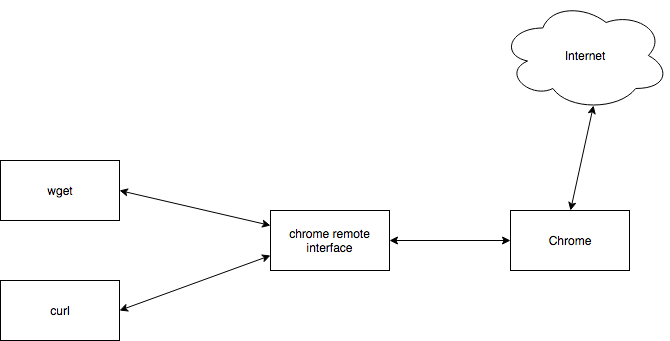
\includegraphics[width=\textwidth]{figures/prototype}
  \caption[Prototype approach]{\textbf{Prototype approach:} Applications issue
  requests and fetch responses from Chrome through the Chrome remote debugging
  protocol. Chrome makes the request on the application's behalf and fetches
  handles all connection security specifics.}
  \label{fig:prototype-saber}
\end{figure}

\subsection{Linking directly to Chrome's networking code}
Using the remote debugging protocol to delegate requests to Chrome is
inefficient since serialized messages are exchanged over a web socket between
the HTTP client and the browser. A more optimized and secure approach would be
to link directly with Chrome's networking library. This could potentially be
more lightweight as it would only require a small subset of Chrome wrapped with
a thin request API that applications could interface with.
\Cref{fig:long-term-saber} shows a potential design for this approach. We leave
this approach for future work.

\begin{figure}[h]
  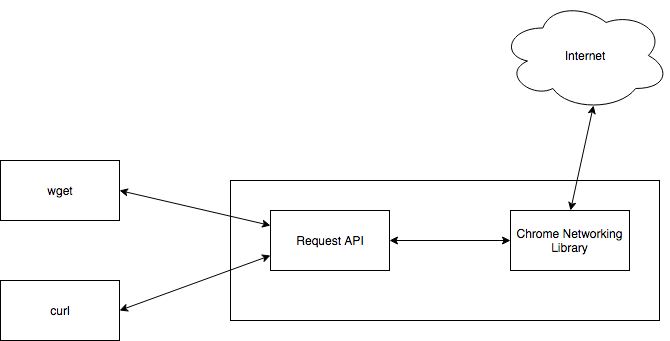
\includegraphics[width=\textwidth]{figures/long-term} \caption[Optimal
  approach]{\textbf{Optimal approach:} The network request library from Chrome
  is exported (along with any security handling logic) and wrapped up in a
  library with an exposed Request API that non-browser applications interface
  with.} \label{fig:long-term-saber}
\end{figure}

\subsection{Motivation}
The motivation behind our delegation approach is based on two key facts: (1)
Browsers are already pioneers of providing secure communication and other
applications can capitalize on that. (2) Writing security critical code is
difficult and we want to minimize the amount of such code that needs to be
written by developers. Currently, any HTTP client would have to include its own
code that either correctly implements the TLS protocol, or uses a TLS library
correctly, both of which have proven to be difficult~\cite{dangerous}. As an
example of our delegation approach, we implement \emph{swget}, a prototype of
wget that provides connection security without writing any TLS verification
code. This pattern can also be used to create a library that provides a simple
Fetch API that any HTTP client could interface with easily.

\section{swget}
\label{sec:swget-saber}

\emph{wget} is a popular command line tool for downloading files from a
webserver. It is frequently used by developers to crawl web pages, download
scripts, and sometimes directly pipe such scripts to the shell (for example,
when installing software such as Node or Bower). While such a practice of
executing code obtained remotely can be dangerous in itself, it is especially a
problem if the security of the connection is compromised by a man-in-the middle
attacker.

\begin{figure}[h]
  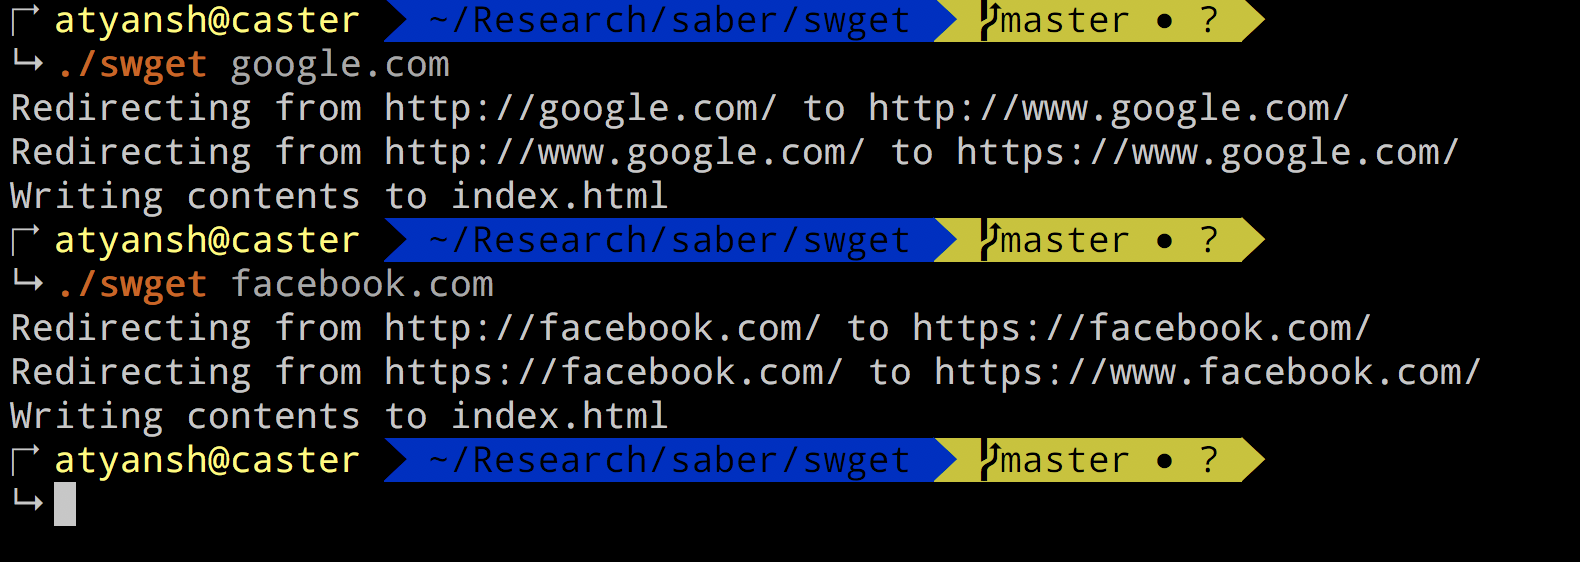
\includegraphics[width=\textwidth]{figures/regular}
  \caption[Regular usage of swget]{swget fetches and saves the webpage similar
  to wget in the normal case}
  \label{fig:regular-saber}
\end{figure}

We wrote our own prototype version of \emph{secure wget} that has the same
basic functionality as wget, but uses Chrome to make network requests.
\Cref{fig:regular-saber} shows standard behavior of swget when fetching a
webpage. Looking at wget's source code, we see it has 994 lines of code for
interfacing with the \emph{OpenSSL} library. Our version of swget does not
require any code to interface with a TLS library. Only 8 lines of code are
needed to add a certificate handler since Chrome would already throw an event
in case any abnormal certificate is encountered. We override Chrome's
certificate handling settings using the remote debugging protocol to grab the
certificate error determined by Chrome and cancel the request. We used the
Chrome remote interface Node.js library to construct our messages to Chrome
which also contributed to the decreased code size. \Cref{fig:cert-error-saber}
shows how swget responds when it catches a certificate error.

\begin{figure}[h]
  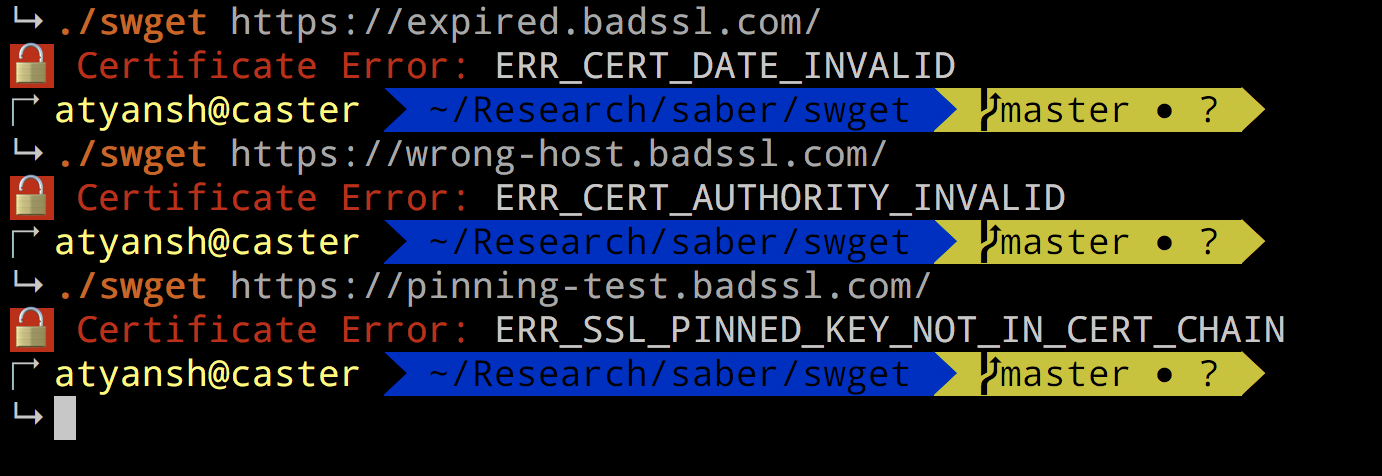
\includegraphics[width=\textwidth]{figures/cert-error}
  \caption[Behavior on certificate errors]{swget catches any certificate errors
  caught by Chrome. In the figure, we see an example of domains with expired
  certificate, mismatched hostname, and an example of website that serves a
  valid certificate that was not pinned as part of the HPKP policy.} 
  \label{fig:cert-error-saber}
\end{figure}


Since Chrome does certificate validation, swget's connection security is at
least as restrictive as that of Chrome by default. We can manually increase or
decrease restrictions based on user supplied arguments to swget. This also
includes protection from revoked certificates, something which wget does not
provide today. A full list of our certificate testing for various clients can
be found in \Cref{tab:results-table-saber}.
\subsection{Secure redirects}

\begin{figure}[H]
  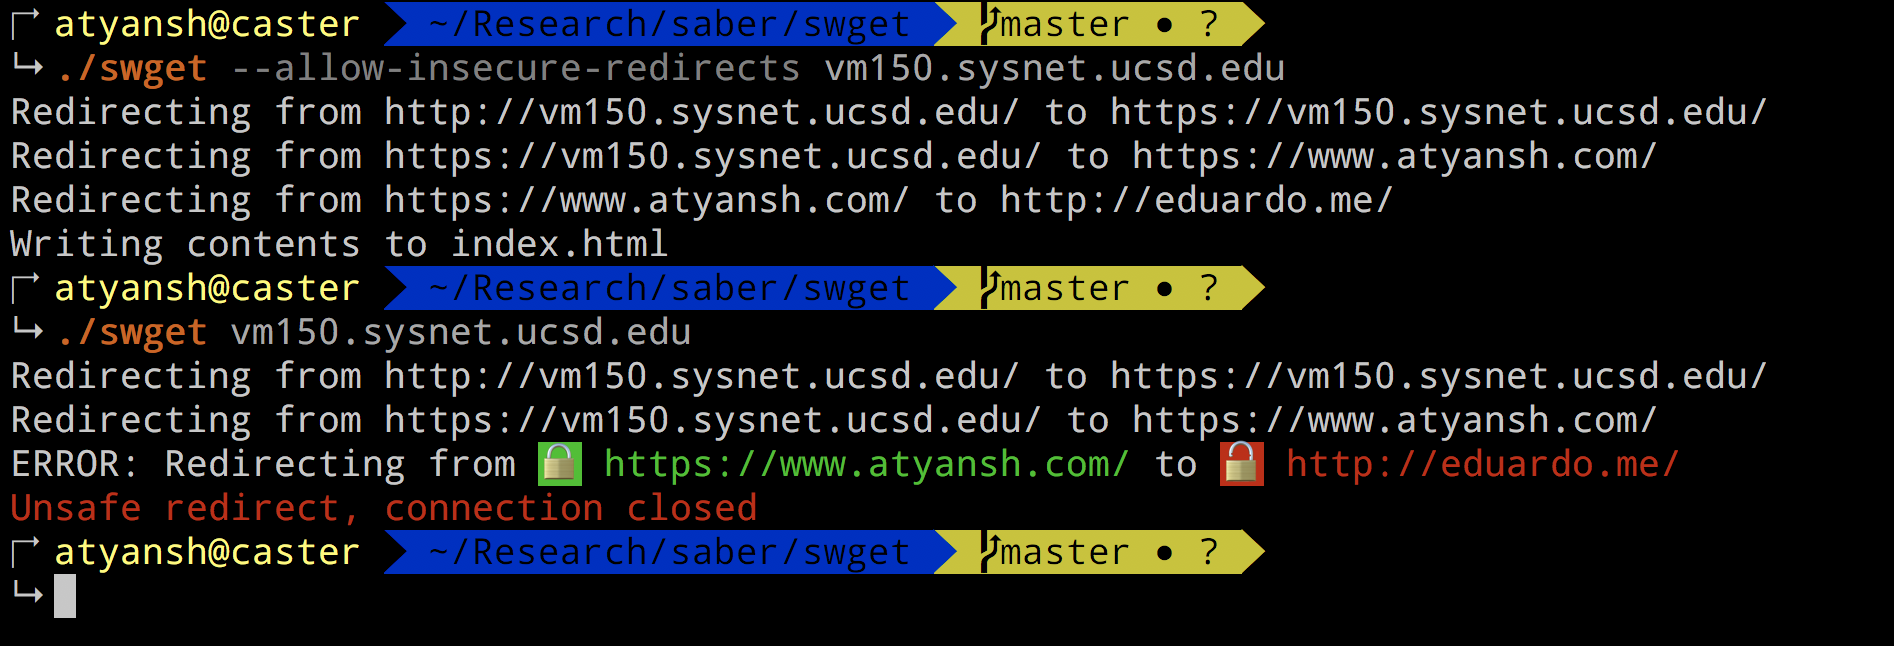
\includegraphics[width=\textwidth]{figures/redirect}
  \caption{Preventing unsafe https to http redirects} 
  \label{fig:redirect-saber}
\end{figure}

The default redirect behavior for Chrome is for top level requests is to follow
redirects. While this behavior is okay for Chrome, this may not be ideal for an
application like wget. Users use wget to fetch and download files. If a request
to fetch was made for an https link which was then redirected to HTTP, security
of the connection could be compromised by an attacker. While browsers can
display the current security status to the user, there's no convenient way to
check whether a file downloaded with wget was actually downloaded securely or
not, once the file has already been fetched. We disable HTTPS to HTTP redirects
by default in our implementation of swget. As seen from
\Cref{fig:redirect-saber} a connection is terminated if the application
encounters an unsafe redirect. Command-line HTTP clients such as wget and curl
do not currently provide secure redirects.

\subsection{Warning messages}
Non-browser applications have suffered from having poor UI in comparison to
browsers. Previous research has shown that better browser TLS warnings
decreased user click-through~\cite{warningland}. We believe that users that use
non-browser applications would similarly benefit from improved warning messages
and have included more visual indicators (such as lock symbols) to convey the
security state of the connection. This is especially noticeable in the case of
redirects (\Cref{fig:redirect-saber}) and malware warnings
(\Cref{fig:malware-saber}). Further work needs to be done to measure the
effectiveness of these warnings.

\begin{figure}[h]
  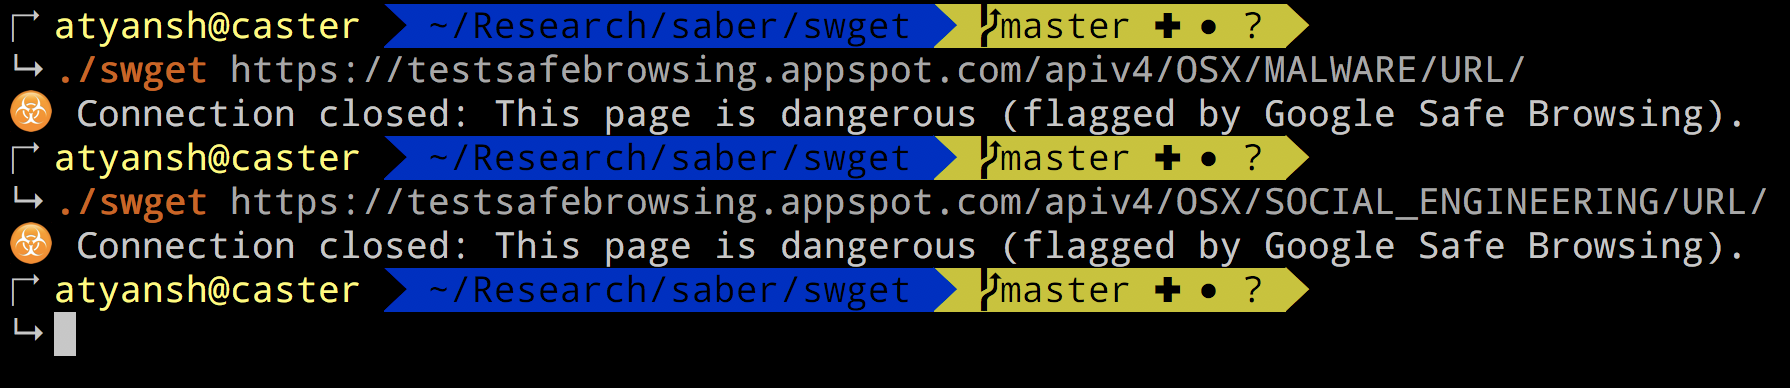
\includegraphics[width=\textwidth]{figures/malware}
  \caption{Malware detection as flagged by Chrome} 
  \label{fig:malware-saber}
\end{figure}

\subsection{Cookies and basic authentication}
Since swget uses Chrome to issue web requests, it can take advantage of
Chrome's session management. This allows us to enable/disable cookies for
swget. Depending on the behavior the user wants, the user's Chrome profile can
be used if the client needs to access the browser cookies, otherwise, a fresh
Chrome user profile could be created that doesn't share any session state with
the user's actual browser.

Cookie authentication can be pretty useful, especially to download web pages
that require authentication (for example, Facebook). In standard wget, the user
would have to provide their login credentials to wget or create a special
authentication token for wget. In case of swget, the browser is already
authenticated with the web server hence no further authentication is needed.

To demonstrate this, we provide an example of HTTP basic authentication by
using swget on a website that requires a user to provide login credentials
before visiting the website. Using wget on this website would return a
\emph{401 Unauthorized} error unless the credentials are provided along with
the url. We used a simple username/password prompt to allow an swget user to
provide credentials dynamically if a website requests for them. Since Chrome
remembers the authentication credentials for the session, any further requests
would automatically have the credentials filled by Chrome. This can be seen in
\Cref{fig:basic-auth-saber}. The user is prompted again if the credentials did
not match correctly.
\begin{figure}[h]
  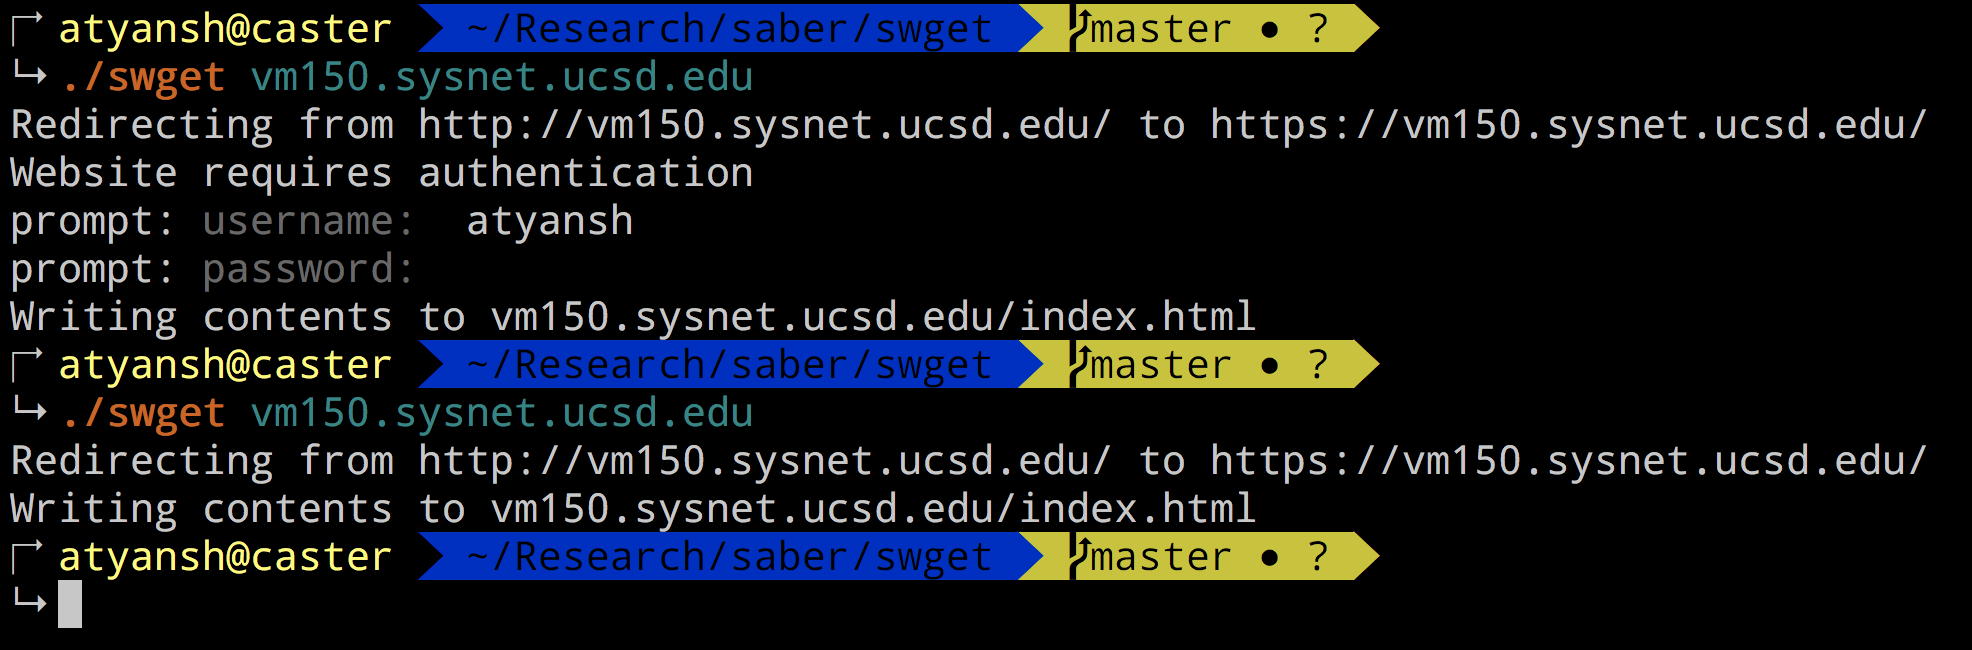
\includegraphics[width=\textwidth]{figures/basic-auth}
  \caption{HTTP Basic Auth} 
  \label{fig:basic-auth-saber}
\end{figure}

\subsection{Centralized HSTS and HPKP}
When Chrome receives an HSTS or HPKP header from a domain, it would record the
header and provide protection for the website. Wget provides a similar HSTS
protection for a domain. However, if an HSTS entry is recorded for a website by
Chrome, the user gets HSTS protection only for Chrome, and not wget, and vice
versa. In fact, any two different clients do not share these protections with
each other. As such, the user is vulnerable every time they make an HTTP
request for a website from a new client even though they have previously
received an HSTS header for the domain via different client. The same
problem exists for HPKP.

The model of delegating connection security to a single client---Chrome in our
prototype---provides a centralized way to maintain HSTS and HPKP records. As such,
any clients (such as swget) automatically share these protections with the
browser. In fact, all clients that use this model would share these
protections.

\subsection{Future Work}
Browsers provide protection against mixed-content in webpages (for example,
HTTP hyperlinks on a webpage served over HTTPS) through security warnings. They
also disable loading HTTP iframes when the top level page is served over HTTPS.
Further, if a \emph{Content-Security-Policy} header is served by the server
that specifies the client to upgrade insecure requests, browsers will upgrade
insecure HTTP requests to HTTPS. Swget currently does not support these
mechanisms but we plan to implement CSP request upgrades in the future.

We also plan to add subresource integrity checking to swget. Browsers can
verify the integrity of subresources downloaded over HTTP, commonly seen for
media downloaded from a CDN, by checking the cryptographic hash of the
subresource obtained over HTTPS. Command-line HTTP clients can benefit greatly
from subresource integrity.

\section{Conclusion}
\label{sec:conclusion-saber}

Today, non-browser HTTP clients are weak to network adversaries in ways that
browsers aren't. Our successful implementation of swget shows that this is a
feasible strategy of building non-browser HTTP clients that require connection
security without interfacing directly with a TLS library.

Another approach involves retrofitting implementations of SSL Libraries
through dynamic linking~\cite{certshim}. The benefits of this approach is that
it doesn't require existing applications to be changed. However, this mechanism
only improves proper certificate validation, it doesn't provide further
protections such as malware detection, HSTS upgrade, browser maintained CRLs,
etc. In contrast, our approach also address protection sharing across clients
through a centralized protection mechanism.

\section{Acknowledgements}
\label{sec:acknowledgement-saber}
\Cref{ch:saber}, in part is currently being prepared for submission for
publication of the material. Jaiswal, Atyansh; Luck, Jonathan; Chao, Joshua;
Shacham, Hovav; Stefan, Deian. The dissertation/thesis author was the primary
investigator and author of this material.
